\section{Tree to Random Forest}
\subsection{Decision Tree}

\begin{frame}
	\frametitle{Decision Tree}
	\framesubtitle{Example}
	\begin{figure}		
		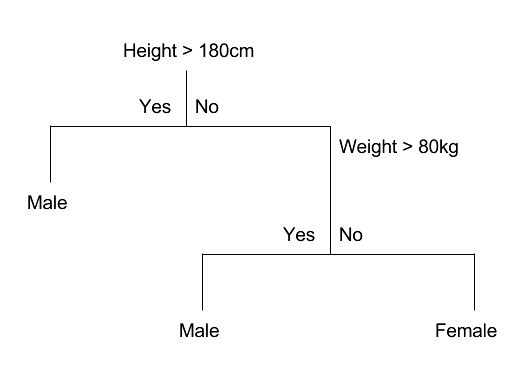
\includegraphics[height=0.7\textheight]{images/decision_tree_example.png}
	\end{figure}
\end{frame}

%%%% Decision Tree: Tree Building Process
\begin{frame}
	\frametitle{Decision Tree: Tree Building Process}
	A tree is grown starting from the root node by repeatedly 
	using the following steps on each node (also called binary splitting):
	\begin{enumerate}
		\item[(i)] \textbf{Find best split \(s\) for each feature \(X_{m}\)}
		\item[(ii)] \textbf{Find the best splitof the node}
		\item[(iii)] \textbf{Repeat until stopping criterion got satisfied}
	\end{enumerate}
\end{frame}	

%%%% Decision Tree: Purity Measures
\begin{frame}
	\frametitle{Decision Tree}
	\framesubtitle{Purity Measures}
	\begin{block}{Gini Measure}
		\begin{equation*}    
			i(t) = \sum_{c \in C} p(c|t) (1 - p(c|t))
		\end{equation*}
	\end{block}
	\begin{block}{Information Entropy}
		\begin{equation*}    
			i(t) = \sum_{c \in C} p(c|t) log(p(c|t))
		\end{equation*}
	\end{block}	
	where $C$ is the set of classes $c$ and $t$ a node of the tree.
\end{frame}
